\section{Design Overview and Pipeline Structure}
The methodology is structured as three sequential, independently cached stages. Each stage produces artefacts---compressed NumPy archives, PyTorch state dictionaries, or CSV result files---that are written to persistent storage before the next stage begins. This design allows the pipeline to be safely interrupted and resumed, a practical requirement given the Colab Pro session time limits described in Chapter 5.

\textbf{Stage A---Per-Modality Encoder Training.} Three independent deep learning models---one for each modality---are fine-tuned or trained from scratch on each subject's EAV data. After training, two artefacts are saved per subject-modality pair: the encoder's full state dictionary, for later feature extraction; and the per-trial test-set logits and labels, for the naive late-fusion baseline and the suppression matrix analysis. These artefacts are the raw material for all downstream stages.

\textbf{Stage B---Pre-Classifier Feature Extraction.} Each trained encoder is loaded, the final classification head is removed, and the penultimate-layer representation is extracted for every training and test trial. The result is three feature matrices per subject---audio, vision, and EEG---each of shape $(N_{\mathrm{trials}}, d_{\mathrm{feature}})$. These cached features allow Stage C to iterate on fusion hyperparameters without re-running the computationally expensive per-modality encoders.

\textbf{Stage C---Fusion Training and Evaluation.} The \texttt{TrimodalAttentionFusion} module is trained on the cached per-subject features. For each subject, the best-test-epoch fusion logits are retained, and per-subject accuracy is appended to a CSV result file. Separately, the per-modality Stage A logits are used to compute a naive late-fusion baseline with no training required and to populate the coherence suppression matrix.

\begin{figure}[htbp]
\centering
\IfFileExists{images/fig_4_1_trimodal_pipeline.png}{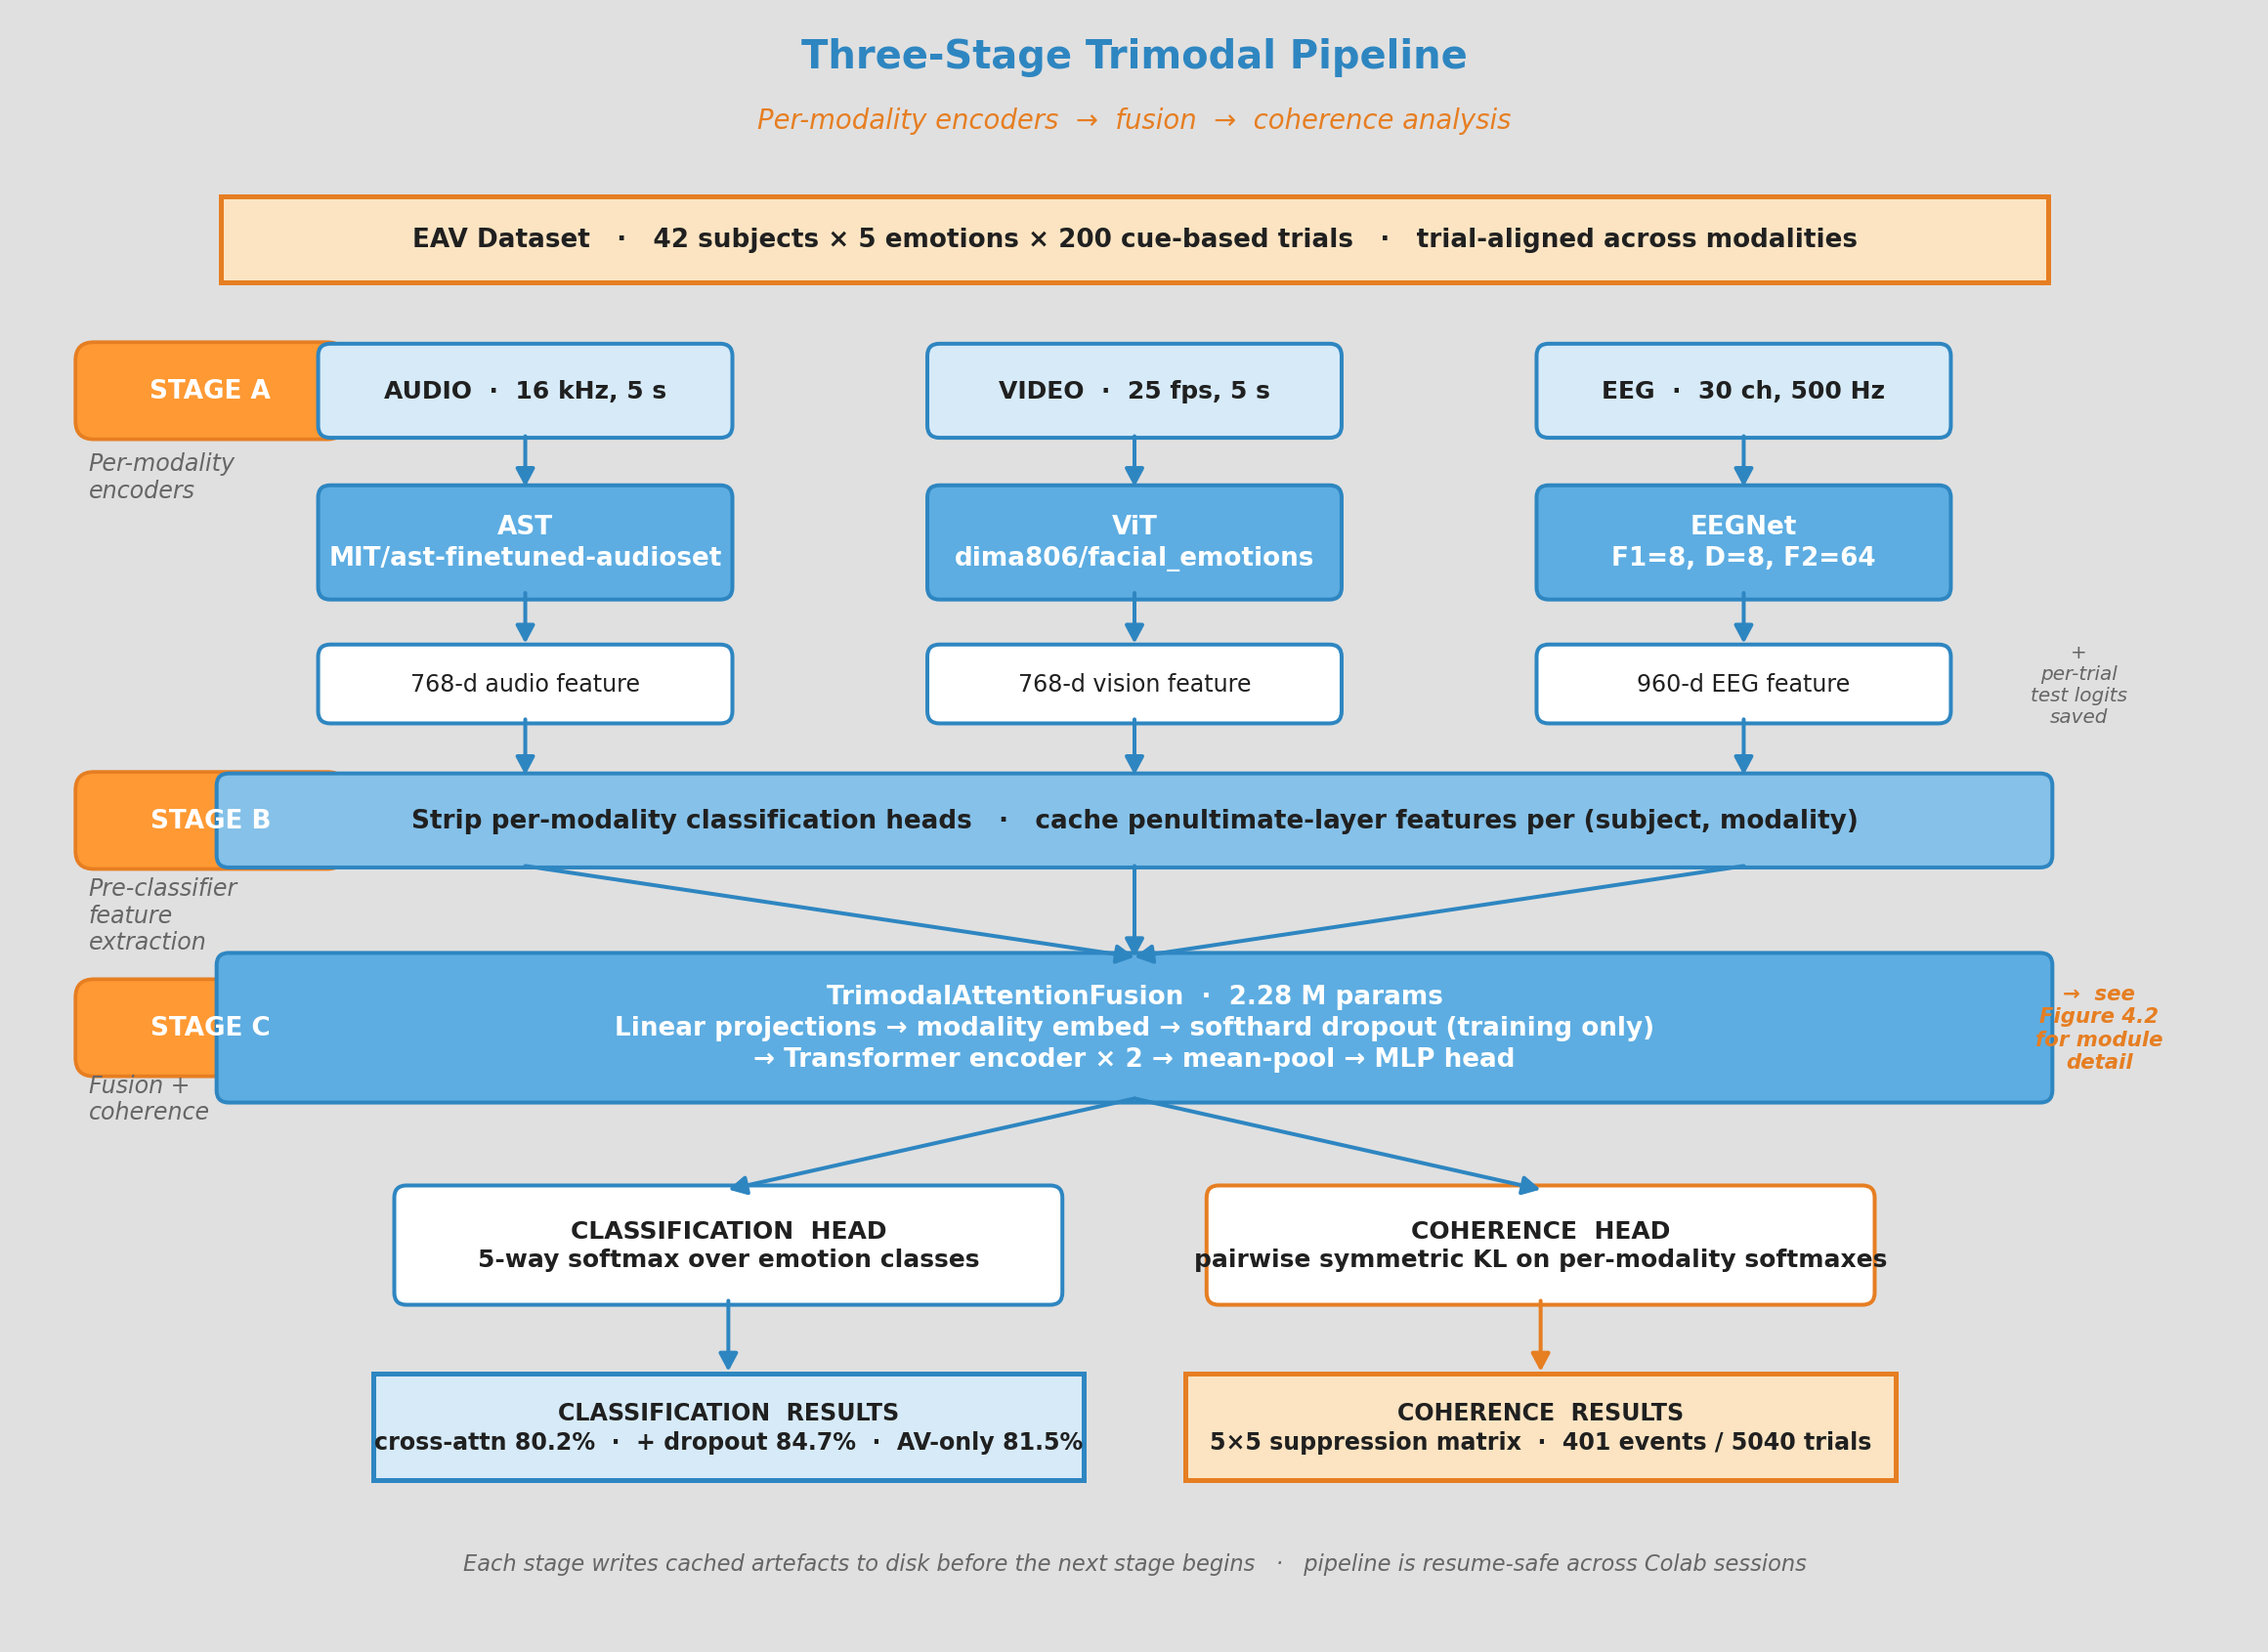
\includegraphics[width=0.9\textwidth]{images/fig_4_1_trimodal_pipeline.png}}{\fbox{\parbox{0.86\textwidth}{\centering Missing image placeholder: \texttt{images/fig\_4\_1\_trimodal\_pipeline.png}. Upload the original pipeline diagram here.}}}
\caption{Three-stage trimodal pipeline: per-modality encoders, cross-modal attention fusion, and coherence analysis.}
\label{fig:trimodal_pipeline}
\end{figure}

Figure \ref{fig:trimodal_pipeline} illustrates the three-stage pipeline. The architecture is designed with two explicit long-term commitments. First, the fusion module's \texttt{forward()} method returns a dictionary containing five named tensors: \texttt{logits}, \texttt{audio\_embed}, \texttt{vision\_embed}, \texttt{eeg\_embed}, and \texttt{fused\_embed}. The per-modality post-attention embeddings are stable outputs under a fixed API contract, enabling a future temporal head (LSTM, Residual-TCN, or temporal transformer) to read them without modifying the fusion module. Second, the \texttt{forward()} signature accepts \texttt{x\_eeg} as a regular argument with no default, but produces finite output when \texttt{x\_eeg} is a zero tensor. This is the architectural guarantee that enables the modality-dropout robustness evaluation in Section \ref{sec:modality_dropout} and the demonstration component.

\section{Dataset: EAV}
\subsection{Corpus Description}
The EAV (EEG-Audio-Video) dataset was published by Lee, Shomanov, Kabidenova, and Yazici at Nazarbayev University in \textit{Scientific Data} \cite{Lee2024EAV}. The corpus covers 42 healthy adult participants in a cue-based, pseudo-random conversation paradigm designed to elicit five target emotions: Neutral, Anger, Happiness, Sadness, and Calmness. Each session records three synchronised streams:

\begin{itemize}
    \item \textbf{EEG:} 30-channel, 500 Hz sampling rate, standard 10--20 electrode placement, acquired with a BrainAmp Standard amplifier.
    \item \textbf{Audio:} 16 kHz mono, recorded concurrently during the participant's spoken responses to each emotion cue.
    \item \textbf{Video:} 30 frames per second, $640\times480$ pixels, capturing the participant's face during spoken responses.
\end{itemize}

The paradigm generates approximately 200 interaction clips per subject, divided into listening segments, from which EEG labels are drawn, and speaking segments, from which audio and video labels are drawn. This Listen/Speak asymmetry is a documented design feature of the corpus: the EEG signal is recorded during the period in which the participant hears the emotion-laden stimulus, while the audio and video signals are recorded during the participant's response. The emotional intent for each trial is the same across modalities because the cue drives both the response and the listening context, but the two windows are temporally offset within the same interaction.

\subsection{Pre-Processing Pipeline}
Raw EAV data is pre-processed into pickle files by the scripts in the official EAV repository. The pre-processing steps for each modality are as follows.

\textbf{EEG pre-processing.} The raw 500 Hz EEG signal is first downsampled to 100 Hz by integer-factor decimation: the signal is reshaped and every fifth sample is selected, without an anti-aliasing prefilter. A fifth-order Butterworth bandpass filter with passband 0.5--45 Hz is then applied at the post-downsample rate; this serves both to remove drift and high-frequency noise, and to attenuate any residual aliasing artefacts introduced by the prior naïve decimation. The filtered signal is segmented into non-overlapping five-second windows, yielding segments of shape 30 channels by 500 samples at the 100 Hz post-downsample rate. Each segment is labelled with the emotion class of the corresponding cue. The \texttt{SELECTED\_CLASSES = [1, 3, 5, 7, 9]} constant selects the five listening-task trials corresponding to the five emotion categories.

\textbf{Audio pre-processing.} Raw audio clips are resampled to 16 kHz via \texttt{torchaudio.transforms.Resample}. Each clip is segmented to exactly five seconds (80{,}000 samples) before being passed to the Hugging Face \texttt{AutoFeatureExtractor} for the AST checkpoint, which produces a 128-bin Log-Mel Spectrogram of shape $(\mathrm{time\_frames}, 128)$. Because the segmentation step enforces a fixed five-second clip length, the AST processor's built-in zero-padding for shorter inputs and truncation for longer inputs is not exercised in this pipeline.

\textbf{Vision pre-processing.} Each EAV speaking-segment video clip is recorded at 30 fps for approximately 20 seconds. From the first 600 source frames (the first 20 seconds), every sixth frame is selected, and the first 25 selected frames are retained. This produces 25 frames at an effective 5 fps, covering the first five seconds of the speaking segment. Each frame is resized to $224\times224$ pixels and then normalised to the model's expected mean and variance by the Hugging Face image processor for the ViT checkpoint.

\subsection{Train/Test Split and Trial-Alignment Heuristic}
\label{sec:split_alignment}
The EAV repository provides a stratified split via \texttt{EAV\_datasplit.py}. The split parameter \texttt{h\_idx=56} divides each subject's trials so that 70\% (280 trials) are assigned to training and 30\% (120 trials) to testing, stratified by class. With five emotion categories, this yields 56 training trials per class and 24 testing trials per class, for totals of 280 and 120 respectively. The complete per-subject inventory is therefore 400 trials across all five classes.

A necessary condition for the suppression matrix analysis is that the audio, vision, and EEG test splits are drawn from the same set of 120 trials, so that comparing per-modality predictions on a given trial index is comparing predictions on the same interaction. A heuristic alignment check was performed on all 42 subjects before the suppression analysis was executed: for every subject, the per-class trial count in the test split was extracted for each of the three modalities and compared. The result for all 42 subjects was a uniform count of 80 trials per class per modality in the combined train+test set ($80\times5=400$ per subject), with the stratified test split producing exactly 24 trials per class (120 total) for each modality. The heuristic passes unanimously, providing the necessary condition for valid cross-modal trial comparison. Table \ref{tab:eav_dataset_structure} summarises the full corpus structure.

\begin{table}[htbp]
\centering
\small
\caption{EAV dataset structural summary.}
\label{tab:eav_dataset_structure}
\begin{tabular}{p{5.2cm} p{8.2cm}}
\hline
\textbf{Property} & \textbf{Specification} \\
\hline
Subjects & 42 (21 male, 21 female) \\
Emotion categories & 5 (Neutral, Anger, Happiness, Sadness, Calmness) \\
Total trials per subject & 400 (80 per class) \\
Training trials & 280 per subject per modality (56 per class) \\
Testing trials & 120 per subject per modality (24 per class) \\
EEG channels & 30 (standard 10--20 placement) \\
EEG original sampling rate & 500 Hz \\
EEG processed sampling rate & 100 Hz after downsampling \\
EEG bandpass filter & Butterworth fifth-order, 0.5--45 Hz \\
EEG segment shape & $(30, 500)$ per trial \\
Audio sampling rate & 16 kHz \\
Video frame rate & 30 fps source; 25 frames at 5 fps used for ViT (every 6th frame; first 25 of the speaking segment) \\
Clip duration & 5 seconds \\
Chance accuracy & 20.0\% for five-class uniform prediction \\
\hline
\end{tabular}
\end{table}

\section{Per-Modality Processing Pipelines}
\subsection{Audio Pipeline: Audio Spectrogram Transformer (AST)}
\textbf{Architecture.} The Audio Spectrogram Transformer \cite{Gong2021AST} is a pure attention architecture for audio classification. AST treats the Log-Mel Spectrogram of an audio clip as a 2D image: it is split into overlapping $16\times16$ patches with stride 10, each patch is linearly projected to a 768-dimensional token embedding, and a standard ViT encoder with 12 attention layers and 12 heads processes the resulting token sequence together with a prepended \texttt{[CLS]} token. The \texttt{[CLS]} token's final-layer representation serves as the clip-level audio feature.

\textbf{Pre-trained checkpoint.} The checkpoint used is \texttt{MIT/ast-finetuned-audioset-10-10-0.4593}, an 87-million-parameter model pre-trained on AudioSet, which contains 2 million weakly labelled audio clips across 527 event categories. The breadth of AudioSet covers ambient sounds, speech, music, and environmental audio, making the pre-trained representation broadly useful for downstream audio tasks including speech emotion recognition.

\textbf{Adaptation to EAV.} The 527-class classification head is discarded. The model is reloaded with \texttt{AutoModelForAudioClassification.from\_pretrained(..., num\_labels=5, ignore\_mismatched\_sizes=True)}, which simultaneously re-initialises the head with a fresh \texttt{Linear(768, 5)} layer and sets \texttt{model.config.num\_labels = 5}. The loss is computed externally as:
\begin{equation}
    \mathcal{L}_{\mathrm{audio}} = \mathrm{CrossEntropyLoss}(z_{\mathrm{audio}}, y),
\end{equation}
where $z_{\mathrm{audio}}$ denotes the model logits. This avoids relying on the model's internal loss path, which would read the old configuration and fail.

\textbf{Training protocol.} Training proceeds in two phases. In the frozen phase, the AST backbone parameters are frozen and only the new five-class head is trained for 5 epochs with Adam, learning rate $10^{-4}$, batch size 8. In the fine-tuning phase, all parameters are unfrozen and training continues for a further 5 epochs with learning rate $10^{-5}$ and batch size 8. The total training budget is 5 frozen + 5 fine-tuning = 10 epochs per subject. Best-checkpoint selection is by test accuracy.

\textbf{Feature extraction.} After training, the \texttt{[CLS]} token representation of dimension 768 is extracted for each test and training trial by running the backbone forward without the classification head. These vectors are saved as the audio feature matrix, of shape $(N_{\mathrm{trials}}, 768)$, for Stage C fusion training.

\subsection{Vision Pipeline: Facial-Emotion Vision Transformer (ViT)}
\textbf{Architecture.} The Vision Transformer \cite{Dosovitskiy2021ViT} processes an image by splitting it into non-overlapping $16\times16$ patches, linearly projecting each patch to a 768-dimensional embedding, and processing the patch-token sequence with a 12-layer, 12-head self-attention encoder. As with AST, the \texttt{[CLS]} token's final-layer representation serves as the clip-level visual feature.

\textbf{Pre-trained checkpoint.} The checkpoint is \texttt{dima806/facial\_emotions\_image\_detection}, a ViT-base model fine-tuned on a composite facial expression dataset for 7-class classification (Angry, Disgust, Fear, Happy, Neutral, Sad, Surprise). The 7-class classification head is replaced using the \texttt{from\_pretrained(num\_labels=5, ignore\_mismatched\_sizes=True)} idiom. This is not merely a convenience: the original EAV vision trainer replaced the head manually by setting \texttt{model.classifier = Linear(hidden, 5)} and \texttt{model.num\_labels = 5}, but did not update \texttt{model.config.num\_labels}. The \texttt{from\_pretrained} idiom resolves this by also updating the configuration.

\textbf{Clip-level representation.} Each five-second clip provides 25 uniformly sampled frames at $224\times224$ pixels. Each frame is independently passed through the ViT backbone to produce a 768-dimensional \texttt{[CLS]} embedding. The 25 per-frame embeddings are then averaged to produce a single 768-dimensional clip-level representation. This bag-of-frames averaging is simple but effective for short five-second clips where the dominant emotional expression is relatively stable.

\textbf{Training protocol.} The backbone is frozen for 3 epochs to initialise the new head, then all parameters are unfrozen for a further 2 fine-tuning epochs. Learning rates are $10^{-4}$ in the frozen phase and $10^{-5}$ in the fine-tune phase, with batch size 8.

\textbf{RAM management.} The original EAV vision trainer pre-processed all frames for a subject in a single operation, building a Python list of approximately 10,000 tensors and invoking \texttt{torch.stack(list).to(device)}. On Colab Free, the stack operation alone consumed approximately 8 GB and silently killed the kernel. The fix processes frames in batches of 64, keeps the stacked batch on CPU, and moves each batch to GPU only at training time via the DataLoader.

\textbf{Feature extraction.} The 768-dimensional clip-level embedding, computed as the mean of 25 per-frame \texttt{[CLS]} tokens, is saved per trial per subject for Stage C.

\subsection{EEG Pipeline: EEGNet}
\textbf{Architecture.} EEGNet \cite{Lawhern2018EEGNet} is a compact depthwise separable CNN designed specifically for EEG signal classification across arbitrary electrode montages. The EEGNet implementation used here is parameterised as follows: $F_1=8$, $D=8$, $F_2=64$, \texttt{kernLength=300}, \texttt{Chans=30}, \texttt{Samples=500}, and \texttt{dropoutRate=0.5}. The forward pass comprises two blocks.

\textbf{Block 1: Temporal and Spatial Filtering.} The input tensor has shape $(B, 1, 30, 500)$.
\begin{enumerate}
    \item \texttt{Conv2d(1, 8, kernel=(1, 300), padding='same')} performs temporal convolution, extracting $F_1=8$ temporal filter responses. Kernel length 300 samples corresponds to a three-second temporal scale at 100 Hz.
    \item \texttt{BatchNorm2d(8)} and ELU activation are applied.
    \item \texttt{DepthwiseConv2d(8, 64, kernel=(30, 1), groups=8)} performs spatial convolution combining information across all 30 channels. The output shape is $(B, 64, 1, 500)$.
    \item \texttt{BatchNorm2d(64)}, ELU, \texttt{AvgPool2d((1, 4))}, and \texttt{Dropout(0.5)} reduce the temporal resolution to 125 samples.
\end{enumerate}

\textbf{Block 2: Pointwise Feature Extraction.} Operating on $(B, 64, 1, 125)$:
\begin{enumerate}
    \item \texttt{Conv2d(64, 64, kernel=(1, 16), padding='same')} performs separable pointwise convolution.
    \item \texttt{BatchNorm2d(64)}, ELU, \texttt{AvgPool2d((1, 8))}, and \texttt{Dropout(0.5)} reduce the temporal resolution to 15 samples.
    \item Flattening produces a vector of length $64\times(500/4/8)=64\times15=960$.
    \item \texttt{Linear(960, 5)} is the final classification head.
\end{enumerate}
The penultimate 960-dimensional flattened representation is the EEG feature vector used in Stage C fusion training.

\textbf{Bug fixes note.} Two EEGNet-specific bugs were identified and resolved during this thesis. The first, a forward-hook implementation defect, caused all EEGNet training to fail with a BatchNorm dimension error. PyTorch's \texttt{register\_forward\_hook} protocol substitutes the hook's return value as the layer's output if the hook returns a non-\texttt{None} tensor. The original EAV repository used lambda hooks in which \texttt{renorm\_} is in-place but returns the modified weight tensor. The lambda propagated this tensor as the hook's return value, and PyTorch replaced the depthwise convolution's output with the weight tensor, causing the downstream BatchNorm to crash. The fix extracts the hook into a named function that returns \texttt{None} explicitly.

A second training bug was identified in the shared trainer: \texttt{self.model.train()} was called once before the outer epoch loop, but \texttt{validate()} called at the end of each epoch switches the model to evaluation mode. From epoch 2 onwards, training was executed with BatchNorm layers in evaluation mode and all Dropout layers disabled. The fix relocates \texttt{self.model.train()} to the beginning of the epoch loop.

Table \ref{tab:encoder_specs} summarises the three encoders.

\begin{table}[htbp]
\centering
\scriptsize
\caption{Per-modality encoder specifications.}
\label{tab:encoder_specs}
\begin{tabular}{p{2.6cm} p{3.5cm} p{3.5cm} p{3.4cm}}
\hline
\textbf{Property} & \textbf{Audio (AST)} & \textbf{Vision (ViT)} & \textbf{EEG (EEGNet)} \\
\hline
Architecture & Pure transformer & Pure transformer & Depthwise separable CNN \\
Pre-training & AudioSet (2M clips, 527 classes) & Facial expressions (7-class) & None; trained from scratch \\
Trainable parameters & 87 million & 86 million & Approximately 2.2 million \\
Input representation & 128-bin Log-Mel Spectrogram & 25 frames of $224\times224$ & $(30, 500)$ EEG segment \\
Output feature & 768-dim \texttt{[CLS]} token & 768-dim mean \texttt{[CLS]} token & 960-dim flattened vector \\
Frozen epochs & 5 & 3 & N/A \\
Fine-tune/full epochs & 5 & 2 & 350 \\
Optimizer/LR & Adam, $10^{-4}$ to $10^{-5}$ & Adam, $10^{-4}$ to $10^{-5}$ & Adam, $10^{-4}$ \\
\hline
\end{tabular}
\end{table}

\section{Trimodal Cross-Modal Attention Fusion Module}
\subsection{Motivation and Design Rationale}
\label{sec:fusion_design_rationale}
The \texttt{TrimodalAttentionFusion} module takes the three per-modality pre-classifier feature vectors as input and produces a five-class emotion prediction plus four auxiliary named embedding outputs. Its design follows from two constraints.

First, the encoders produce single pooled vectors per clip rather than token sequences. Given that each modality contributes exactly one token representation per clip, the feature resolution available to the fusion module is limited to single pooled vectors.

Second, the reference architecture \cite{Lee2024MERCL} employs six directional pairwise cross-modal attention operations: audio-to-vision, vision-to-audio, vision-to-EEG, EEG-to-vision, audio-to-EEG, and EEG-to-audio. This design is motivated by sequence-level modality representations produced by residual-TCN encoders. At single-token-per-modality resolution, pairwise cross-attention reduces algebraically to a learned linear projection. Self-attention over a three-token sequence performs the same cross-modal mixing at this resolution, with cleaner code, fewer parameters, and no loss of expressive power.

\subsection{Architectural Specification}
The complete forward pass of \texttt{TrimodalAttentionFusion} proceeds through five stages, illustrated in Figure \ref{fig:attention_architecture}.

\begin{figure}[htbp]
\centering
\IfFileExists{images/fig_4_2_attention_arch.png}{
\includegraphics[width=0.9\textwidth]{images/fig_4_2_attention_arch.png}}{\fbox{\parbox{0.86\textwidth}{\centering Missing image placeholder: \texttt{images/fig\_4\_2\_attention\_architecture.png}. Upload the original TrimodalAttentionFusion architecture diagram here.}}}
\caption{TrimodalAttentionFusion architecture: per-modality linear projections to $D=256$, modality-type embeddings, two-layer transformer encoder, mean pooling, and MLP classification head.}
\label{fig:attention_architecture}
\end{figure}

\textbf{Stage 1---Per-Modality Projection.} Three independent linear layers project the modality-specific feature vectors to a common embedding dimension $D=256$:
\begin{equation}
\begin{aligned}
    h_a &= W_a x_a + b_a, && x_a \in \mathrm{R}^{768}, \\
    h_v &= W_v x_v + b_v, && x_v \in \mathrm{R}^{768}, \\
    h_e &= W_e x_e + b_e, && x_e \in \mathrm{R}^{960},
\end{aligned}
\end{equation}
where $a$, $v$, and $e$ denote audio, vision, and EEG respectively. The projections are independent, allowing each modality's raw feature space to be transformed by a projection tailored to its statistics.

\textbf{Stage 2---Modality-Type Embedding.} A learnable parameter matrix $E_{\mathrm{mod}}\in\mathrm{R}^{3\times256}$ is initialised to small random values with $\sigma=0.02$ and added element-wise to the projected vectors. Index 0 is added to the audio projection, index 1 to the vision projection, and index 2 to the EEG projection:
\begin{equation}
    u_m = h_m + E_{\mathrm{mod}}[m].
\end{equation}
These embeddings serve the same role as positional embeddings in a sequence transformer, enabling the attention mechanism to learn modality-specific attention patterns.

\textbf{Stage 3---Transformer Encoder.} The three 256-dimensional modality tokens are stacked into a sequence:
\begin{equation}
    U = [u_a; u_v; u_e] \in \mathrm{R}^{B\times3\times256},
\end{equation}
and processed by a two-layer transformer encoder with 8 attention heads, feedforward dimension 1024, GELU activation, Pre-LayerNorm normalisation, and dropout 0.1. After the transformer encoder, a final \texttt{LayerNorm(256)} is applied to the output sequence.

\textbf{Stage 4---Mean Pooling.} The three post-attention tokens are averaged across the sequence dimension to produce a single fused representation:
\begin{equation}
    f = \frac{1}{3}\sum_{m\in\{a,v,e\}} \tilde{u}_m,
\end{equation}
where $\tilde{u}_m$ denotes the post-transformer token for modality $m$. This fused vector is returned as \texttt{fused\_embed}; the three unpooled tokens are returned separately as \texttt{audio\_embed}, \texttt{vision\_embed}, and \texttt{eeg\_embed}.

\textbf{Stage 5---MLP Classification Head.} The fused representation is passed through:
\begin{equation}
    z = W_2\,\mathrm{Dropout}\left(\mathrm{GELU}(W_1 f + b_1)\right) + b_2,
\end{equation}
producing the raw five-class logit vector. Cross-entropy loss is computed on these raw logits during training.

The module has approximately 2,285,573 trainable parameters: 638,976 in projection layers, 768 in modality embeddings, approximately 1,577,984 in the two-layer transformer encoder, 512 in post-normalisation, and 67,333 in the MLP head.

\subsection{Architectural Guarantee: Finite Output Under Zero-EEG Input}
A formal contract test embedded in the module verifies the zero-EEG inference property:

\begin{verbatim}
out_zero = model(x_audio, x_vision, torch.zeros(B, 960))
assert torch.isfinite(out_zero["logits"]).all()
assert out_zero["logits"].norm() > 0.01
\end{verbatim}

When $x_e$ is a zero tensor, Stage 1 produces:
\begin{equation}
    h_e = W_e\cdot 0 + b_e = b_e.
\end{equation}
Stage 2 then adds the EEG modality embedding:
\begin{equation}
    u_e = b_e + E_{\mathrm{mod}}[e].
\end{equation}
This is a deterministic but non-trivial vector. The transformer can therefore learn, during modality-dropout training, to suppress the zero-EEG token's contribution to the fused embedding when only audio and vision are present. The guarantee is architectural, not learned: it holds even before modality-dropout training.

\begin{table}[htbp]
\centering
\small
\caption{TrimodalAttentionFusion hyperparameters and training configuration.}
\label{tab:fusion_hyperparameters}
\begin{tabular}{p{5.4cm} p{7.8cm}}
\hline
\textbf{Hyperparameter} & \textbf{Value} \\
\hline
Common embedding dimension & $D=256$ \\
Modality-type embedding shape & $(3, 256)$ \\
Transformer encoder layers & 2 \\
Attention heads per layer & 8 \\
Feedforward dimension & 1024 \\
Activation & GELU \\
Normalisation & Pre-LayerNorm (\texttt{norm\_first=True}) \\
Dropout & 0.1 in attention and feedforward sublayers \\
MLP head & \texttt{Linear(256, 256)} $\rightarrow$ GELU $\rightarrow$ Dropout(0.1) $\rightarrow$ \texttt{Linear(256, 5)} \\
Total trainable parameters & Approximately 2.28 million \\
Fusion training epochs & 80 \\
Optimiser & AdamW \\
Learning rate & $10^{-3}$ \\
LR schedule & Cosine annealing \\
Batch size & 32 \\
\hline
\end{tabular}
\end{table}

\section{Naive Late-Fusion Baseline}
The naive late-fusion baseline provides the primary comparison point for the \texttt{TrimodalAttentionFusion} module. It requires no learned parameters and operates directly on the per-modality test logits saved during Stage A.

For each subject and each test trial index $t$, the computation is:
\begin{equation}
    p_m(t) = \mathrm{softmax}(z_m(t)), \quad m\in\{a,v,e\},
\end{equation}
\begin{equation}
    \bar{p}(t) = \frac{p_a(t)+p_v(t)+p_e(t)}{3},
\end{equation}
\begin{equation}
    \hat{y}(t) = \arg\max_k \bar{p}_k(t).
\end{equation}
The mean-softmax variant is the canonical choice because it treats each modality as an independent vote weighted by its confidence, without requiring any learning of modality weights. Two alternative variants are also implemented but not reported as primary results: sum-of-log-softmax, equivalent to the product-of-probabilities rule, and hard majority voting with tie-breaking by confidence.

Any fusion architecture that fails to beat mean-softmax averaging is providing no measurable benefit beyond what can be obtained by treating the three modalities as three independent, equally weighted experts. In EAV's within-subject, 280-training-trial regime, this turns out to be a stringent comparison point. Beyond accuracy, the baseline script computes the symmetric KL divergence between each pair of per-modality softmax distributions for each test trial, saving them for the coherence analysis in Section \ref{sec:coherence_analysis}.

\section{Cross-Modal Affective Coherence Analysis}
\label{sec:coherence_analysis}
The suppression matrix is computed from the per-modality test-set predictions pooled across all 42 subjects' 120 test trials each, for a total of 5,040 trials.

A trial $t$ from subject $s$ qualifies as a suppression event if and only if:
\begin{equation}
S(s,t)=1 \Longleftrightarrow
\begin{cases}
\hat{y}_{a}(s,t)=\hat{y}_{v}(s,t), & \text{external audio-vision consensus},\\
\hat{y}_{e}(s,t)\neq\hat{y}_{a}(s,t), & \text{internal EEG divergence},\\
\max_k p_{e,k}(s,t)\geq0.5, & \text{confident EEG prediction}.
\end{cases}
\end{equation}
Condition 1 ensures that a clear external signal exists. Conditions 2 and 3 together ensure that a confident, internally divergent signal also exists. The threshold 0.5 is conservative: it requires EEG to place more probability mass on one class than on all other four classes combined, before the divergence is counted as a suppression event. Trials failing any condition are excluded from the matrix.

\begin{figure}[htbp]
\centering
\IfFileExists{images/fig_4_3_suppression_criteria.png}{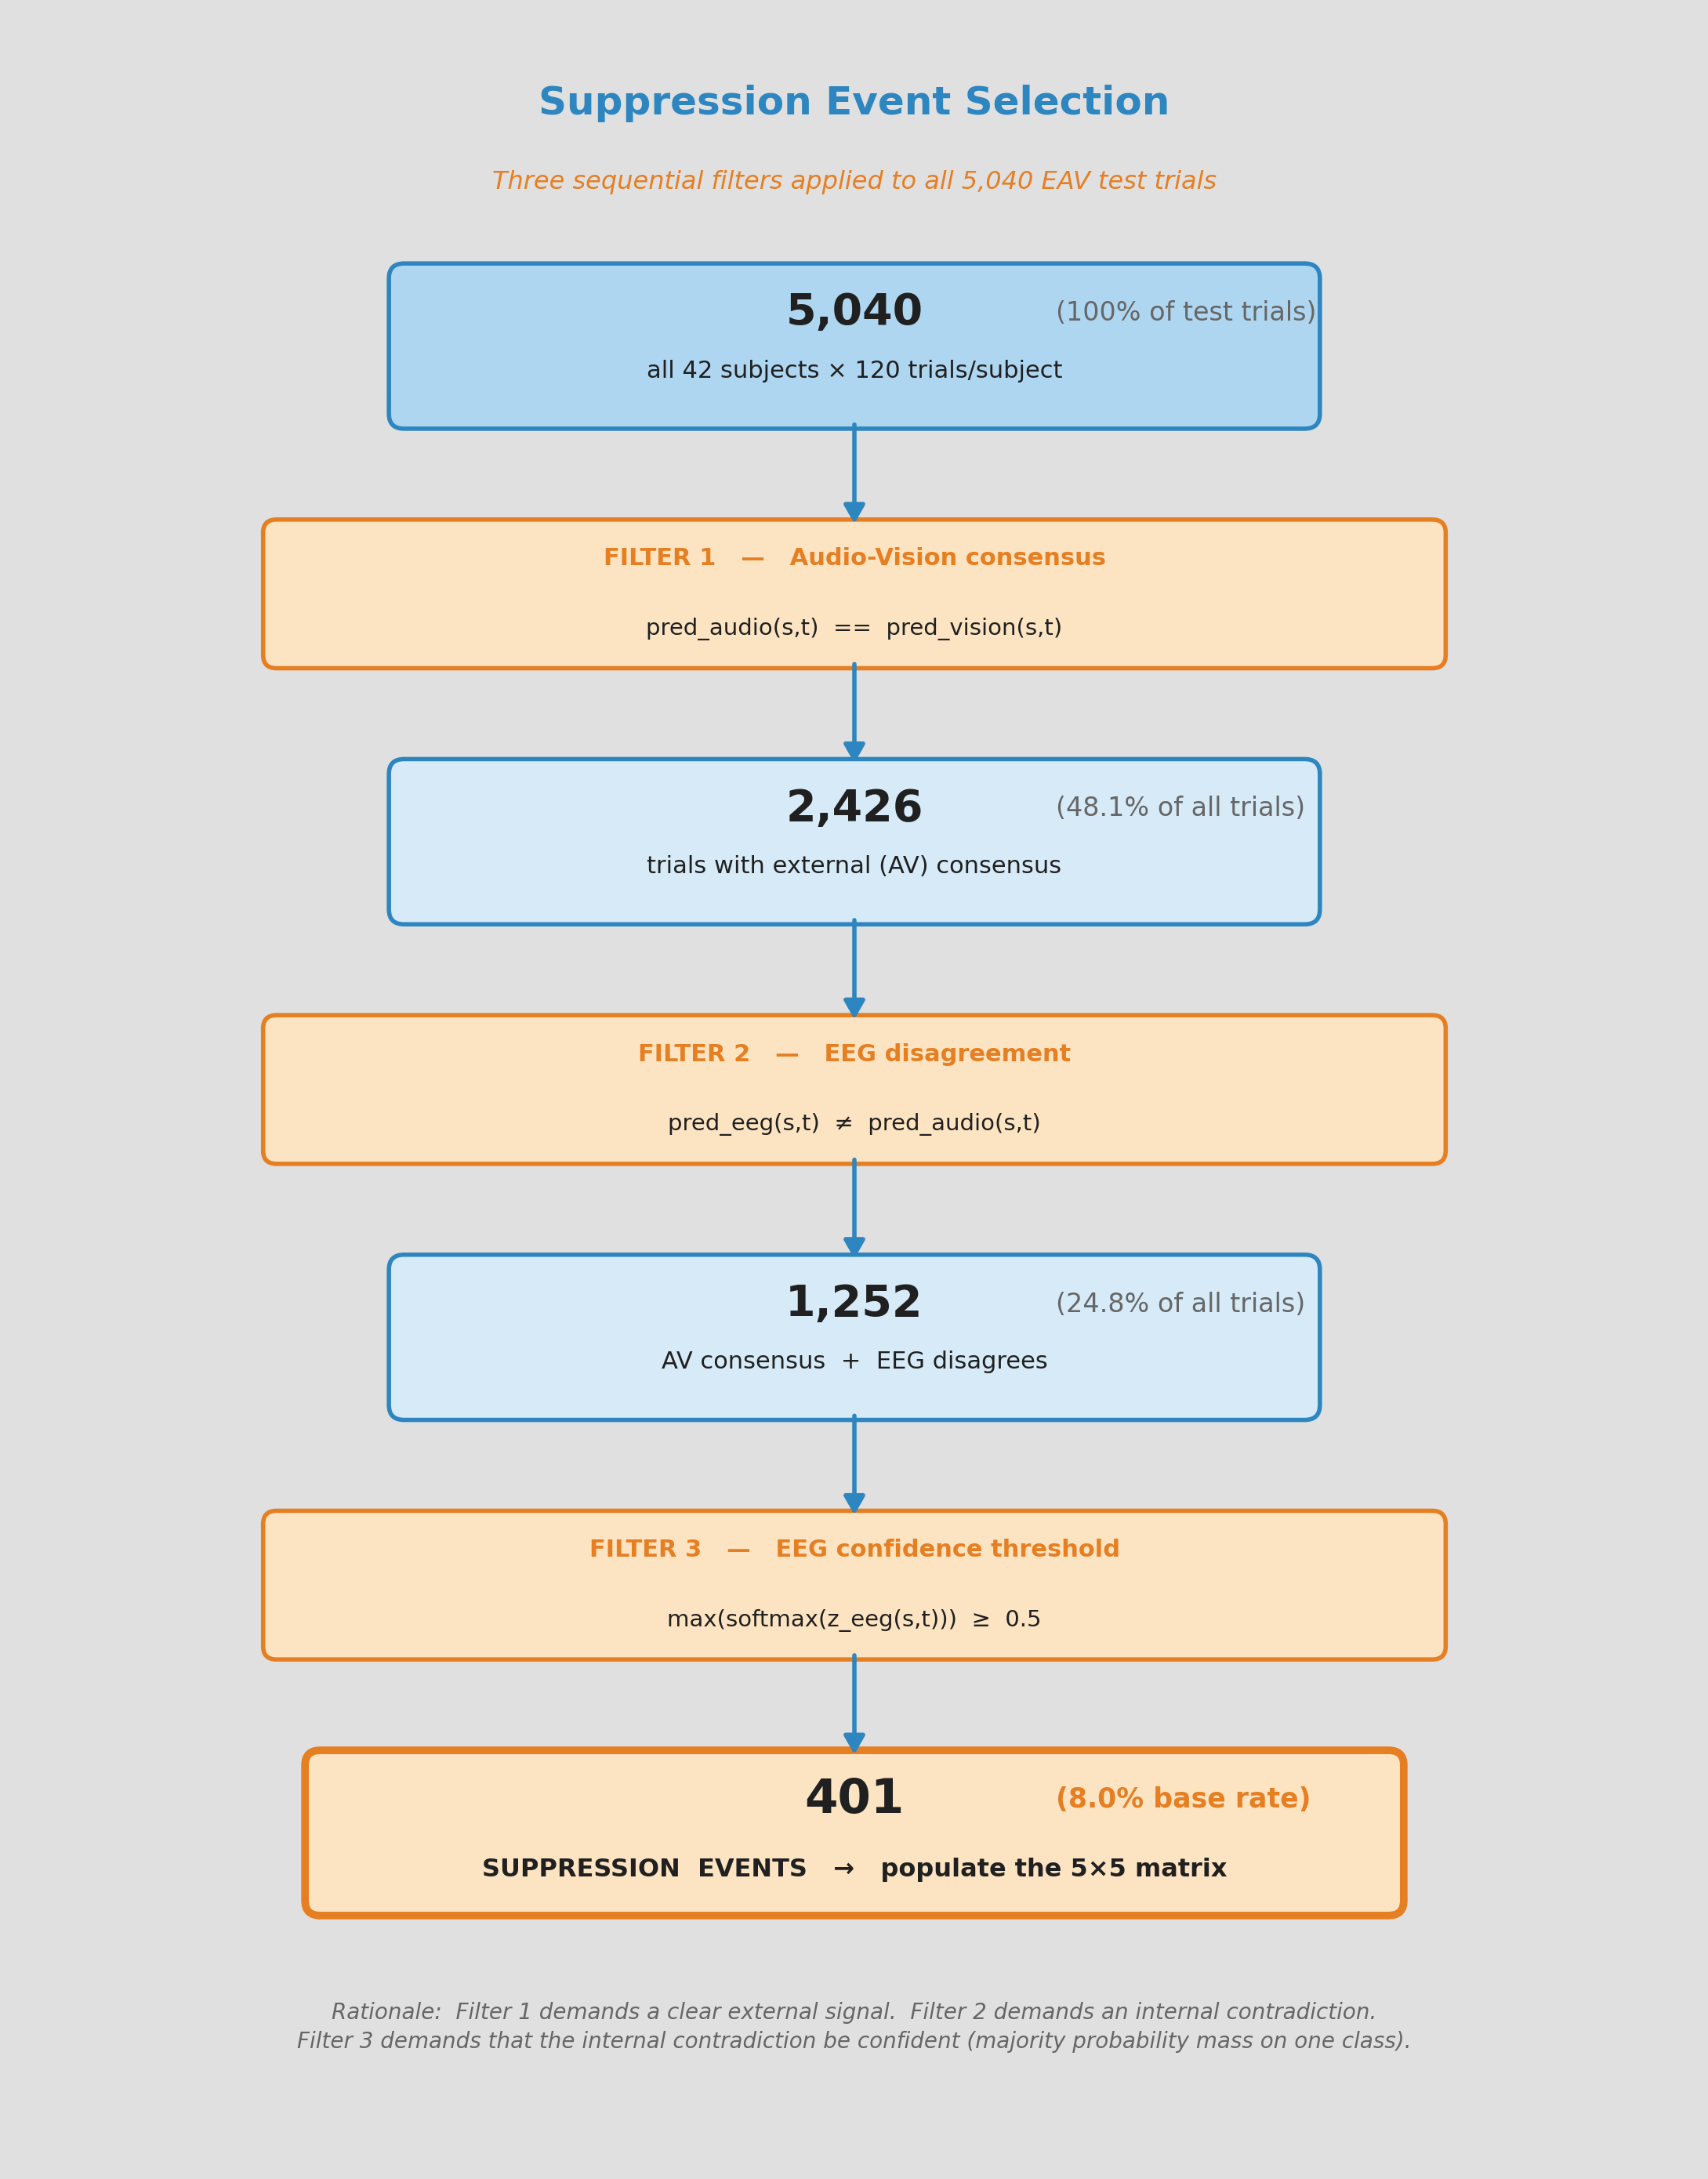
\includegraphics[width=0.9\textwidth]{images/fig_4_3_suppression_criteria.png}}{\fbox{\parbox{0.86\textwidth}{\centering Missing image placeholder: \texttt{images/fig\_4\_3\_suppression\_criteria.png}. Upload the original suppression-event criteria diagram here.}}}
\caption{Suppression event selection criteria: audio-vision consensus on emotion class $E_{av}$, EEG prediction $E_{eeg}\neq E_{av}$, and EEG top-1 confidence $\geq0.5$.}
\label{fig:suppression_criteria}
\end{figure}

Each qualifying trial contributes a unit count to cell $(r,c)$ of the $5\times5$ matrix, where $r=\hat{y}_{a}(s,t)$ is the external consensus row index and $c=\hat{y}_{e}(s,t)$ is the internal EEG prediction column index:
\begin{equation}
    M_{r,c}=\sum_{s=1}^{42}\sum_{t=1}^{120}\mathbf{1}\left[S(s,t)=1 \land \hat{y}_{a}(s,t)=r \land \hat{y}_{e}(s,t)=c\right].
\end{equation}
The diagonal is zero by construction because EEG agreement with the external consensus is excluded by the second criterion.

To verify that matrix patterns are cross-population rather than driven by individual outlier subjects, the per-subject contribution to each cell is extracted. A pattern is classified as cross-population if it is contributed by more than five distinct subjects and no single subject contributes more than 40\% of the cell total.

\section{Modality Dropout and Robustness}
\label{sec:modality_dropout}
To enable meaningful inference when EEG is unavailable---as will be the case in any deployment scenario without an EEG headset---the fusion module is trained under a modality-dropout regime adapted from Chumachenko, Iosifidis and Gabbouj \cite{Chumachenko2022SelfAttention}.

The softhard dropout scheme expands each training batch into four sub-batches:
\begin{itemize}
    \item \textbf{Full modality:} audio, vision, and EEG features are used as-is.
    \item \textbf{Audio-only:} vision and EEG features are replaced by zero tensors.
    \item \textbf{Vision-only:} audio and EEG features are replaced by zero tensors.
    \item \textbf{Audio-visual:} EEG features are replaced by a zero tensor, while audio and vision are used as-is.
\end{itemize}
For each subject's training batch of $N$ trials, this produces an expanded batch of $4N$ trials. The labels are replicated identically across all four sub-batches. The module is therefore trained on examples in which any combination of the three modalities may be absent, forcing the learned projections and attention weights to develop predictions robust to modality absence.

The audio-visual sub-batch, with EEG zeroed and audio and vision present, is the most important for the demonstration use case, in which EEG is unavailable but audio and video are present. The module learns to produce accurate predictions under this condition specifically, in addition to maintaining accuracy on the full-modality case. After modality-dropout training, the zero-EEG inference accuracy across all 42 subjects is the primary robustness metric. This metric is the number reported on the demonstration overlay as ``EEG unavailable; prediction uses audio + video only.''